\chapter{骨格情報}\label{abst}
本研究では,Kinectを用いて骨格情報の取得を行った.本章では,Kinectと骨格情報について詳しく述べて行く.

\section{Kinectの概要}
Kinectは,Microsoft社が開発したXbox360用のコントローラの一つである.ハードウェア機能として,
RGBカメラ,距離カメラ,4つのマイクを並べたマイクアレイがある.その中でも,距離カメラは,Kinectから赤外線を照射し,
その反射を読み取ることで利用者を認識し,骨格の情報を認識することができる.骨格を認識,追跡することにより,
利用者の動きを3次元データで取得することが可能である.Kinectを骨格の認識,追跡をするために設置するときは,
高さ60cmから180cmの間に設置し,利用者の全身がカメラに収まるようにする.Kinectの垂直視野角は43度,水平視野角は57度である.
実際に使用する際は,頭から膝上のあたりまでが画面に入れば認識されるが,全身が画面に入ったほうがより精度が向上する.
図\ref{fig:Kinect}は実際に使用したKinectと同じ種類のものである.

\begin{figure}[htbp]
  \begin{center}
    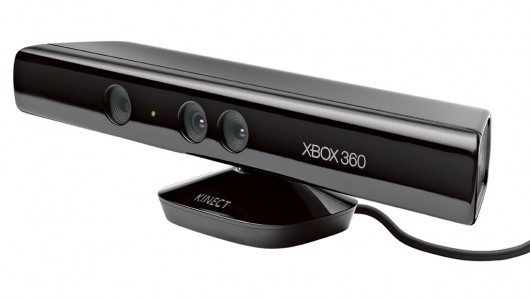
\includegraphics[clip,width=7.0cm]{./images/Kinect.jpg}
    \caption{Kinect}
    \label{fig:Kinect}
  \end{center}
\end{figure}

\newpage

\section{骨格情報の取得}
Kinectを使用して骨格情報を取得する.Microsoft社が公開したソフトウェア開発キットである
Kinect for Windows SDK (以下SDK)[2]を用いることにより,音声を含めてKinectに搭載されている各種センサのデータを取得することができる.
また,SDKは骨格座標の取得が可能であり,図\ref{fig:kokkaku}のように,体の中心線上の4箇所と,両手足の関節位置16箇所の合計20箇所が取得できる.
骨格座標は3次元データの位置情報をメートル単位で取得でき,30fpsで計測される.分解能は,x成分,y成分が2mの場所で3mm,z成分が1cmである.
Kinectで取得した骨格座標をもとに分析を行っていく.
\begin{figure}[htbp]
  \begin{center}
    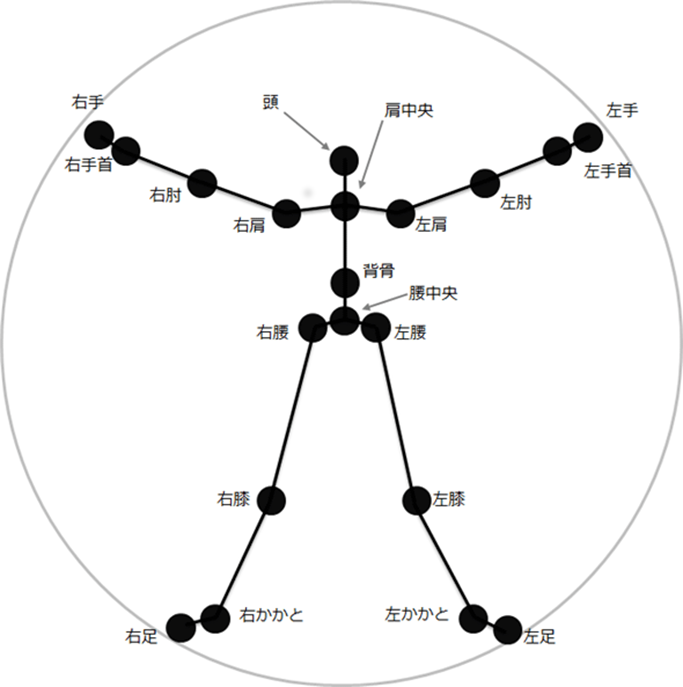
\includegraphics[clip,width=7.0cm]{./images/kokkaku.png}
    \caption{SDKで取得可能な関節点}
    \label{fig:kokkaku}
  \end{center}
\end{figure}